% \section{Priliminary}
\section{Preliminary}
% \subsection{Multi-turn Tool-Integrated Reinforcement Learning}
We denote the query by $\x$, the tool feedback by $\ob$, and the model’s action by $\y$. For a given query $\x$, the model autoregressively generates an action at turn $t$ according to
\[
\pi_{\theta}\!\left(\y_t \mid \x, \y_0, \ob_0, \y_1, \ldots, \ob_{t-1}\right),
\]
where $\y_t$ is produced based on the accumulated context, and $\ob_{t-1} \sim \mathcal{T}$ denotes the tool feedback returned at turn $t-1$ if the previous action $\y_{t-1}$ invoked a tool $\mathcal{T}$ (e.g., issuing a search query). If no tool is invoked, $\ob_{t-1}$ is an empty string.
The \textit{multi-turn} setting thus corresponds to trajectories involving multiple tool calls. However, tool feedback $\mathbf{o}_t$ is inherently out-of-distribution (OOD) for the LLM, as it originates from external environments rather than the model’s generative distribution. Thus, prior work~\citep{jin2025search} masks feedback tokens during training to stabilize optimization.
\\
\textbf{Tool-Integrated GRPO with Feedback Mask.}
GRPO, introduced in DeepSeek-Math~\citep{shao2024deepseekmath} and DeepSeek-R1~\citep{guo2025deepseek} and later applied to tool use~\citep{jin2025search}, is a value-free policy optimization method with group-relative reward normalization.
Specifically, for a query–answer pair $(\x, \ab)$, the policy $\pi_\theta$ samples $G$ responses:  
\[
\left\{(\y_{i,0},\ob_{i,0},\ldots,\y_{i,t},\ob_{i,t},\ldots,\ob_{i,T_i-1},\y_{i,T_i}) \right\}_{i=1}^G,
\]
where $T_i$ denotes the number of tool calls, and thus determines the number of multi-turn interactions in the $i$-th rollout.  
Each action $\y_{i,t}$ consists of $|\y_{i,t}|$ tokens, and we denote by $\y_{i,t,<k}$ the prefix consisting of its first $k-1$ tokens. Let $r_i$ denote the reward assigned to the $i$-th response.  
The advantage for the $t$-th action of $i$-th response is defined via group-level normalization:
\[
\hat{A}_{i,t,k} := \frac{r_i - \mu}{\sigma}, \qquad k = 1, \ldots, |\hat{\y}_{i,t}|,
\]
where $\mu = \widehat{\mathbb{E}}[\{r_i\}_{i=1}^G]$ and $\sigma = \sqrt{\widehat{\mathrm{Var}}[\{r_i\}_{i=1}^G]}$ are the empirical mean and standard deviation of rewards within the group.  
Each token of the same trajectory shares the same normalized advantage. The tool-integrated GRPO objective \textbf{with feedback mask} is given by:
\begin{align}\label{eq:grpo}
& \mathcal{J}_{\mathrm{GRPO}}(\theta) = 
\mathbb{E}_{\substack{(\x,\ab)\sim\mathcal{D} \\ \{ (\y_{i,t},\ob_{i,t})_{t=0}^{T_i-1},\y_{i,T_i}\}\sim ( \pi_{\theta_{\mathrm{old}},\mathcal{T}})}} \nn \\
 & 
\Bigg[
\frac{1}{\sum_{i=1}^{G} \sum_{t=1}^{T_i} |\hat{\y}_{i,t}|}
\sum_{i=1}^{G} \sum_{t=1}^{T_i} \sum_{k=1}^{|\hat{\y}_{i,t}|}
 \min\!\Bigl(
\gamma_{i,t,k}(\theta)\,\hat{A}_{i,t,k},\;
\nn \\
& \hat{A}_{i,t,k}\,\mathrm{clip}\big(\gamma_{i,t,k}(\theta),\,1-\varepsilon,\,1+\varepsilon\big)
\Bigr)
\Bigg],
\end{align}
where $\varepsilon$ is the clipping parameter, the likelihood ratio is defined as
$\gamma_{i,t,k}(\theta)= \frac{\pi_\theta(\y_{i,t,k} \mid \x, \ldots,\y_{i,t-1},\ob_{i,t-1}, \y_{i,t,<k})}
{\pi_{\theta_{\mathrm{old}}}(\y_{i,t,k} \mid \x, \ldots,\y_{i,t-1},\ob_{i,t-1},\y_{i,t,<k})}
$. Although feedback tokens $\ob$ are masked out, they still influence the context of subsequent token predictions.
\begin{figure}[t]
\centering
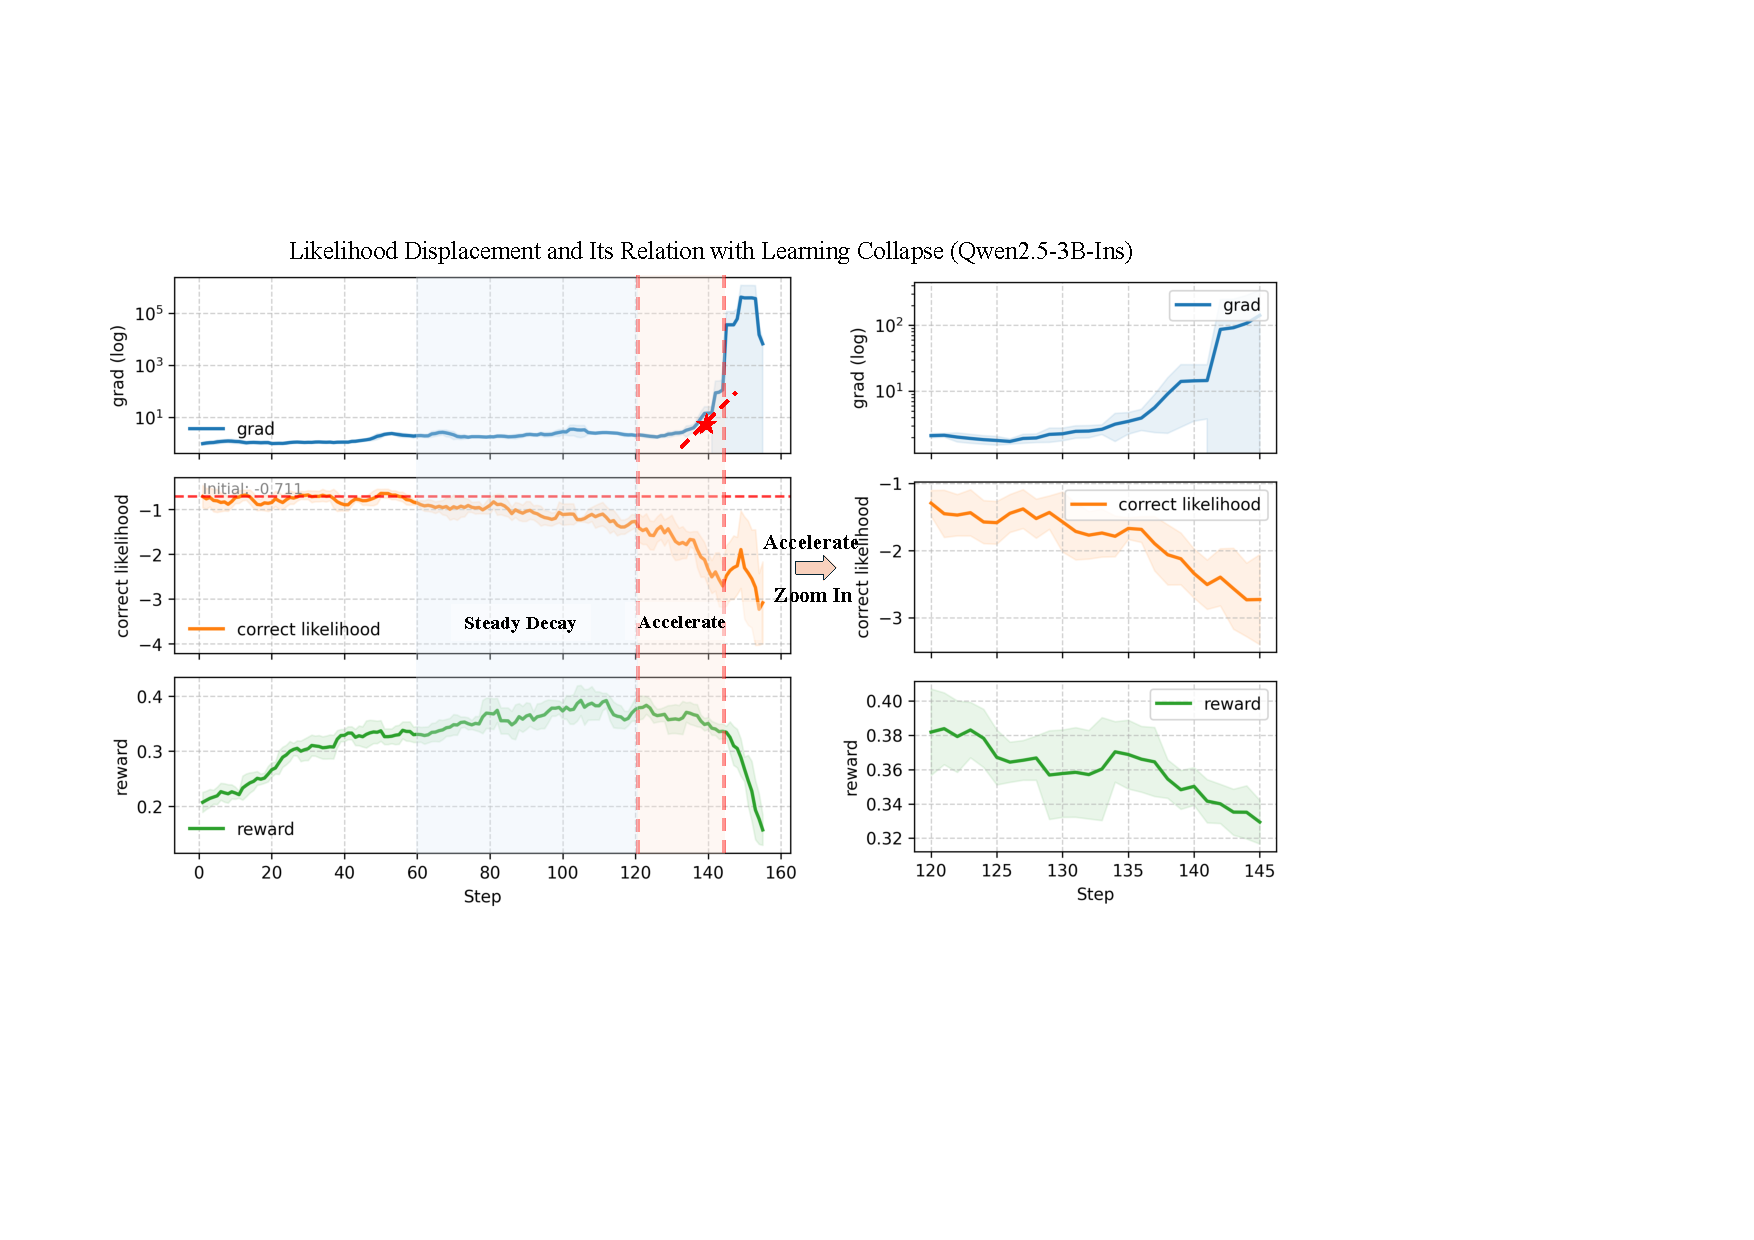
\includegraphics[width=\linewidth]{images/LLD_Tool_dynamic_v2.pdf}
\caption{We illustrate the likelihood displacement in tool-integrated RL training. The steady-decay phase (60-120) emerges even when the reward increases. In the subsequent acceleration phase (after step 120), the likelihood of correct responses drops sharply, accompanied by a sudden surge in gradient magnitude (\textcolor{red}{red star}), leading to gradient explosion. A zoomed-in view of the acceleration region further highlights this effect, showing a clearer likelihood displacement, where the gradient accelerates rapidly while the reward starts to decline. }
\label{fig:dynamic}
\vspace{-4mm}
\end{figure}
\section{Lazy Likelihood Displacement in Tool-integrated GRPO}
% Recent work~\citep{deng2025effect} introduces \textbf{Lazy Likelihood Displacement (LLD)} in GRPO for text-based, non-tool settings, showing that the likelihood of some correct responses improves marginally or even decreases during optimization. In this section, we extend LLD to the tool-integrated RL regime and define \xl{This positions this paper as an extension of LLD to tool-integrated GRPO), making it sound incremental.  }:
We identify a critical but previously unrecognized failure mode in tool-integrated GRPO, in which likelihood displacement progressively accelerates through compounding low-confidence responses and ultimately destabilizes training. While \cite{deng2025effect} identifies LLD as a training pathology in single-turn GRPO, their analysis is restricted to closed-loop text generation without external observations. In contrast, tool-integrated reinforcement learning fundamentally changes the learning dynamics: LLD becomes a trajectory-level instability that interacts with out-of-distribution tool feedback and prefix-shared decision branches, leading to systematic likelihood decay, gradient amplification, and eventual training collapse.

We further show that this phenomenon arises from two structural factors unique to the tool-integrated GRPO setting (analyzed in Section~\ref{sec:correct-actions}) and consistently leads to catastrophic collapse behavior. We formalize and define LLD in the tool-integrated RL regime in this section.
% \begin{definition}\label{def:lld}
% Let $\pi_{\theta_{\text{\rm old}}}$ and $\pi_{\theta_{\text{\rm fin}}}$ denote the initial and final models obtained before and after optimizing a preference-learning objective $\mathcal{J}$ (e.g.,~\cref{eq:grpo}) over a dataset $\mathcal{D}$, such that $\mathcal{J}(\theta_{\text{\rm fin}}) < \mathcal{J}(\theta_{\text{\rm old}})$. We say that \textbf{LLD} occurs for a tuple $(\mathbf{x},\y^+) \in \mathcal{D}$ if, for some small constant $\epsilon \ge 0$,
% \begin{equation}
% \ln \pi_{\theta_{\text{\rm fin}}}(\y^+ \mid \mathbf{x}) 
% \;<\;
% \ln \pi_{\theta_{\text{\rm old}}}(\y^+ \mid \mathbf{x}) + \epsilon .
% \end{equation}
% \end{definition}

% In the setting of \emph{tool-integrated} RL, LLD becomes substantially more severe. Because the loss is computed \emph{only over response tokens}—with all intermediate feedback $\ob$ being masked—the optimization pressure concentrates exclusively on response segments. As a result, instances with $\epsilon = 0$, where the likelihood of correct responses fails to improve at all, appear with striking frequency. This indicates an especially acute form of LLD. Even more troubling, the likelihood of \emph{incorrect} responses also decreases throughout training due to negative gradients, causing a \textbf{progressive decay in the model’s overall output likelihood}. This compounding decay is a distinctive failure mode of tool-integrated RL, where masked feedback prevents gradients from stabilizing the response space.


\begin{definition}[Tool-LLD]\label{def:lld}
Let $\pi_{\theta_{\mathrm{old}}}$ and $\pi_{\theta_{\mathrm{fin}}}$ denote the initial and finetuned policies obtained before and after optimizing the objective $\mathcal{J}$ (e.g.,~\Cref{eq:grpo}) over a dataset $\mathcal{D}$, with $\mathcal{J}(\theta_{\mathrm{fin}}) < \mathcal{J}(\theta_{\mathrm{old}})$.
Consider a tool-integrated trajectory consisting of alternating actions and feedback,
$(\y_{0}, \ob_{0},\; \y_{1}, \ob_{1},\;\ldots,\;\y_{T}),$
where only the actions $\{\y_t\}_{t=0}^{T}$ are used in likelihood computation (feedback is masked).  
For each response action $\y_t$, define its log-likelihood change as
\begin{align}
\Delta_t(\mathbf{x},\y_t)
&:=
\ln \pi_{\theta_{\mathrm{fin}}}(\y_t \mid \mathbf{x},\y_{<t},\ob_{<t}) 
\nonumber \\ &-
\ln \pi_{\theta_{\mathrm{old}}}(\y_t \mid \mathbf{x},\y_{<t},\ob_{<t}). \nonumber
\end{align}
We say that LLD occurs for the action $t$ if  
$\Delta_t(\mathbf{x},\y_t) \;\le\; \epsilon$,
where $\epsilon$ is a small or non-positive constant. And LLD occurs for the whole response if 
\begin{equation}
\sum_{t=0}^T \Delta_t(\mathbf{x},\y_t) \;\le\; \epsilon,
\end{equation}
Therefore, LLD accounts for the failure scenario where \textbf{even correct response actions fail to boost confidence (or even reduce it)} when such an enhancement is explicitly required by the loss function.
\end{definition}
\begin{figure*}[t]
\centering
% ---------- (a): first three ----------
\begin{subfigure}{0.73\textwidth}
    \centering
    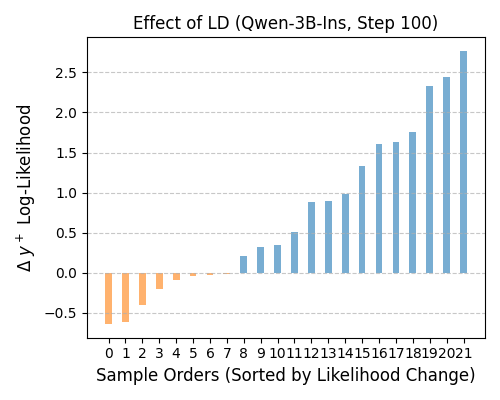
\includegraphics[width=0.32\textwidth]{images/Effect_of_LD/100.png}
    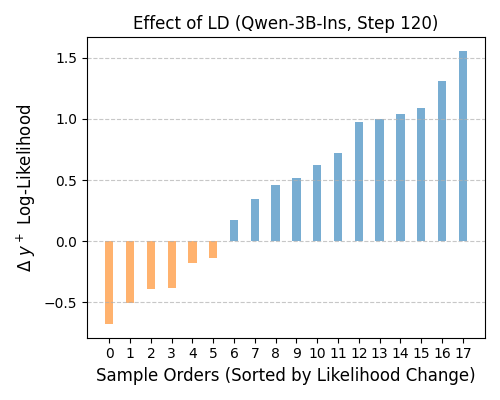
\includegraphics[width=0.32\textwidth]{images/Effect_of_LD/120.png}
    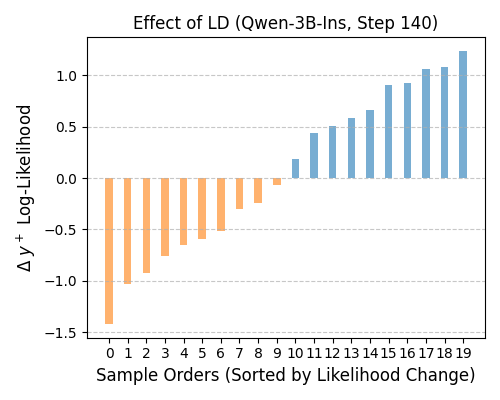
\includegraphics[width=0.32\textwidth]{images/Effect_of_LD/140.png}
    \caption{Likelihood displacement across training steps.}
    \label{fig:effect_ld_a}
\end{subfigure}
\hfill
% ---------- (b): last one ----------
\begin{subfigure}{0.25\textwidth}
    \centering
    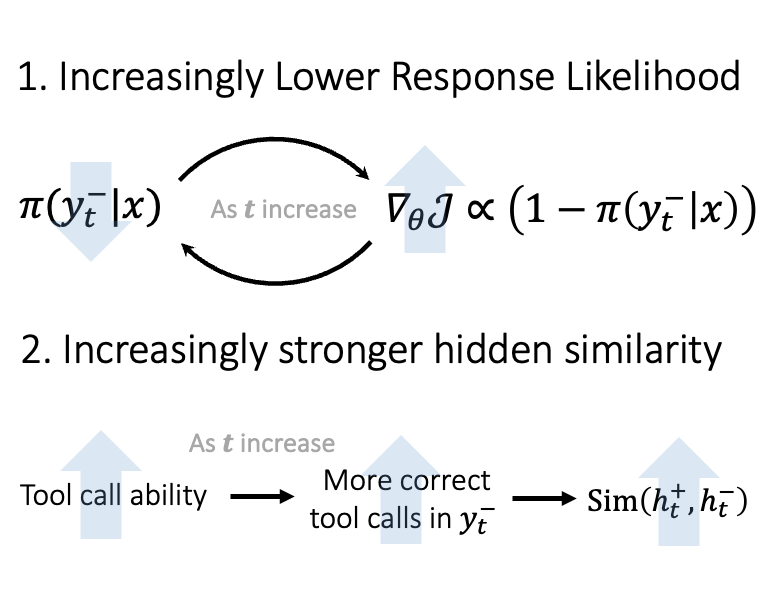
\includegraphics[width=\textwidth]{images/llds2.png}
    \caption{Mechanism}
    \label{fig:effect_ld_b}
\end{subfigure}
\vspace{-2.5mm}
\caption{(a) Effect of likelihood displacement across different training iterations for the Qwen2.5-3B-Instruct model. Results are computed on the first 50 samples of the training set, discarding cases where all responses are uniformly correct or uniformly incorrect. Bars below zero (\textcolor{orange}{orange}) indicate samples whose correct responses' likelihood decreases after training. (b) Illustration of the mechanism: as training progresses, the likelihood of correct responses decreases while hidden-state similarity increases, leading to stronger LLDS.}
\label{fig:effect_of_ld}
\vspace{-6mm}
\end{figure*}
We generalize the negative-gradient characterization of group-relative updates in~\cite{deng2025effect} to a multi-turn setting with external observations, where the learning dynamics differ qualitatively. We present the following informal theorem (Formal statement and proof in~\cref{sec:the_p}).
% \begin{theorem}[Informal: Trajectory-Level LLD in Tool-Integrated GRPO]\label{the:infom}
% In tool-integrated GRPO, the likelihood of an otherwise correct response can \emph{decrease} when
% \emph{(i)} incorrect responses of low likelihood and
% \emph{(ii)} incorrect responses whose embeddings closely resemble the correct one
% induce large negative gradients that dominate the positive updates.
% These forces jointly lead to trajectory-level Lazy Likelihood Displacement.
% \end{theorem}
\begin{theorem}[Informal: Trajectory-Level LLD in Tool-Integrated GRPO]\label{the:infom}
In tool-integrated GRPO, the likelihood of a correct response action can decrease when incorrect responses satisfy two conditions:
\emph{(i) Low likelihood:} The model assigns low probability to incorrect responses, causing large prediction-error weights that magnify their influence, and
\emph{(ii) High embedding similarity:} Incorrect responses share similar representations with correct ones, causing negative gradients to interfere with positive updates. As they frequently do in tool-integrated settings (see Section~\ref{sec:correct-actions}), negative gradients dominate, causing LLD.
\end{theorem}
\vspace{-3mm}
In the setting of tool-integrated GRPO,  we observed \textbf{with striking frequency} that the likelihood of correct responses reduces (\cref{fig:dynamic}). This indicates an especially acute form of LLD ($\epsilon \leq 0$), causing a \textbf{progressive decay in the model’s output likelihood}. This compounding decay is a distinctive failure mode of Search-R1 style TIRL.